% Adapted from the author's soutenance/frangi_termes.tex.
% Same three geometric vignettes, translated into English and made legible.
% Rejection crosses removed: the paper uses soft similarity penalties.
\documentclass[tikz,border=6pt]{standalone}
\usepackage{fontspec}
\setmainfont{EB Garamond}
\usepackage{amsmath}
\usepackage{unicode-math}
\setmathfont{Latin Modern Math}
\usetikzlibrary{arrows.meta}
\definecolor{navy}{RGB}{56,66,87}
\definecolor{red}{RGB}{230,51,18}
\definecolor{teal}{RGB}{0,117,128}
\begin{document}
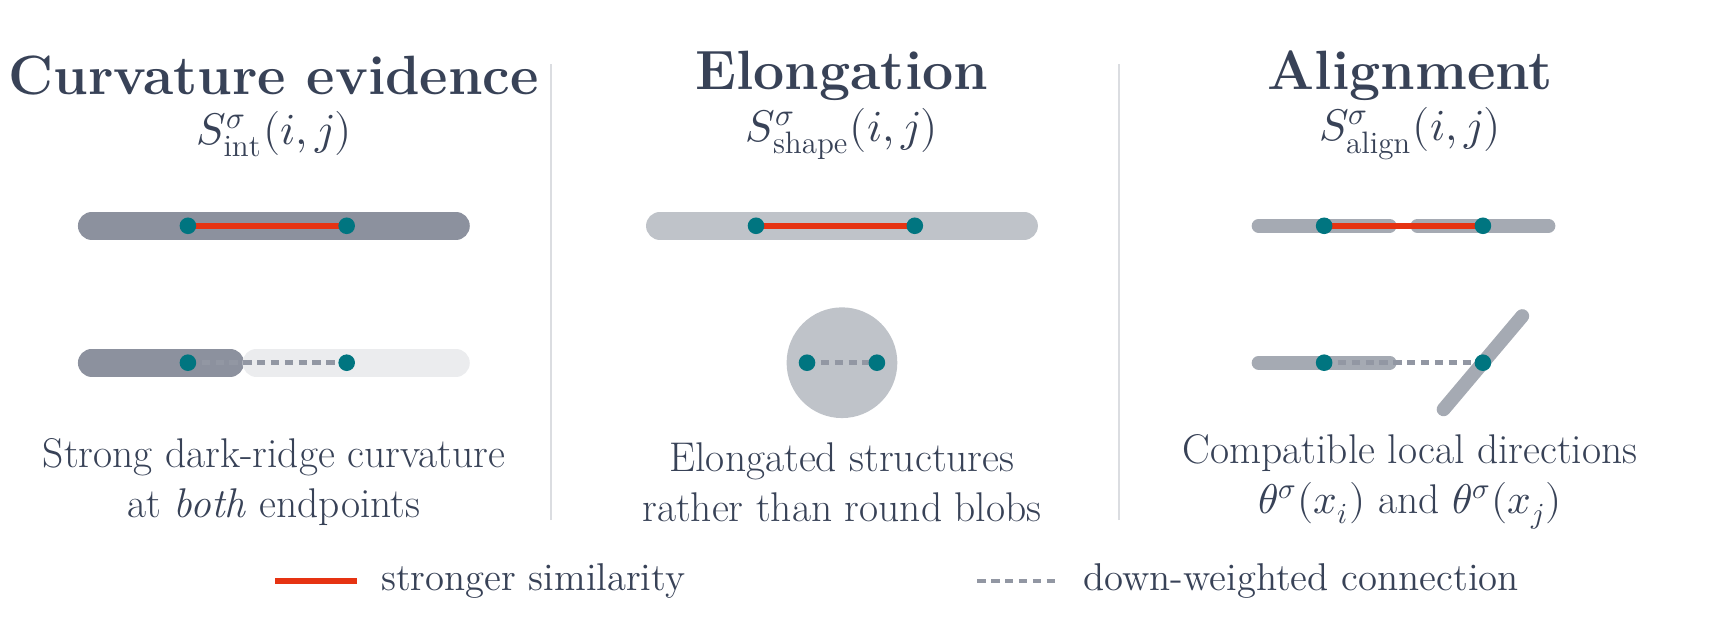
\begin{tikzpicture}[x=1.85cm,y=1.85cm,
 every node/.style={font=\fontsize{16}{19}\selectfont,text=navy},
 ridge/.style={line width=10pt,navy!32,line cap=round},
 pixel/.style={circle,fill=teal,inner sep=0pt,minimum size=6pt},
 strong/.style={red,line width=2.2pt},
 weak/.style={navy!55,line width=1.6pt,densely dashed},
 heading/.style={font=\fontsize{20}{23}\selectfont\bfseries},
 caption/.style={align=center,font=\fontsize{15}{18}\selectfont}]
 \path[use as bounding box] (-.04,-1.57) rectangle (11.44,2.40);
 % Light separators preserve the original three-column organization.
 \draw[navy!18,line width=.8pt] (3.55,-.98)--(3.55,2.15);
 \draw[navy!18,line width=.8pt] (7.45,-.98)--(7.45,2.15);
 \begin{scope}
  \node[heading] at (1.65,2.07) {Curvature evidence};
  \node at (1.65,1.67) {$S_{\mathrm{int}}^\sigma(i,j)$};
  \draw[ridge,navy!58] (.40,1.04)--(2.90,1.04);
  \draw[strong] (1.06,1.04)--(2.15,1.04);
  \node[pixel] at (1.06,1.04) {};
  \node[pixel] at (2.15,1.04) {};
  \draw[ridge,navy!58] (.40,.10)--(1.35,.10);
  \draw[ridge,navy!10] (1.53,.10)--(2.90,.10);
  \draw[weak] (1.06,.10)--(2.15,.10);
  \node[pixel] at (1.06,.10) {};
  \node[pixel] at (2.15,.10) {};
  \node[caption] at (1.65,-.72)
       {Strong dark-ridge curvature\\at \emph{both} endpoints};
 \end{scope}
 \begin{scope}[shift={(3.9,0)}]
  \node[heading] at (1.65,2.07) {Elongation};
  \node at (1.65,1.67) {$S_{\mathrm{shape}}^\sigma(i,j)$};
  \draw[ridge] (.40,1.04)--(2.90,1.04);
  \draw[strong] (1.06,1.04)--(2.15,1.04);
  \node[pixel] at (1.06,1.04) {};
  \node[pixel] at (2.15,1.04) {};
  \fill[navy!32] (1.65,.10) circle[radius=.38];
  \draw[weak] (1.41,.10)--(1.89,.10);
  \node[pixel] at (1.41,.10) {};
  \node[pixel] at (1.89,.10) {};
  \node[caption] at (1.65,-.72)
       {Elongated structures\\rather than round blobs};
 \end{scope}
 \begin{scope}[shift={(7.8,0)}]
  \node[heading] at (1.65,2.07) {Alignment};
  \node at (1.65,1.67) {$S_{\mathrm{align}}^\sigma(i,j)$};
  \draw[navy!45,line width=5pt,line cap=round] (.61,1.04)--(1.51,1.04);
  \draw[navy!45,line width=5pt,line cap=round] (1.70,1.04)--(2.60,1.04);
  \draw[strong] (1.06,1.04)--(2.15,1.04);
  \node[pixel] at (1.06,1.04) {};
  \node[pixel] at (2.15,1.04) {};
  \draw[navy!45,line width=5pt,line cap=round] (.61,.10)--(1.51,.10);
  \draw[navy!45,line width=5pt,line cap=round] (1.88,-.22)--(2.42,.42);
  \draw[weak] (1.06,.10)--(2.15,.10);
  \node[pixel] at (1.06,.10) {};
  \node[pixel] at (2.15,.10) {};
  \node[caption] at (1.65,-.72)
       {Compatible local directions\\$\theta^\sigma(x_i)$ and $\theta^\sigma(x_j)$};
 \end{scope}
 % The drawings indicate a relative response, not a thresholded decision.
 \draw[strong] (1.66,-1.40)--(2.22,-1.40);
 \node[anchor=west,font=\fontsize{14}{17}\selectfont] at (2.32,-1.40)
       {stronger similarity};
 \draw[weak] (6.48,-1.40)--(7.04,-1.40);
 \node[anchor=west,font=\fontsize{14}{17}\selectfont] at (7.14,-1.40)
       {down-weighted connection};
\end{tikzpicture}
\end{document}
